\documentclass{standalone}
\usepackage{tikz}
\usetikzlibrary{patterns, positioning}
\usepackage[sfdefault]{ClearSans} %% option 'sfdefault' activates Clear Sans as the default text font
\usepackage[T1]{fontenc}

\begin{document}
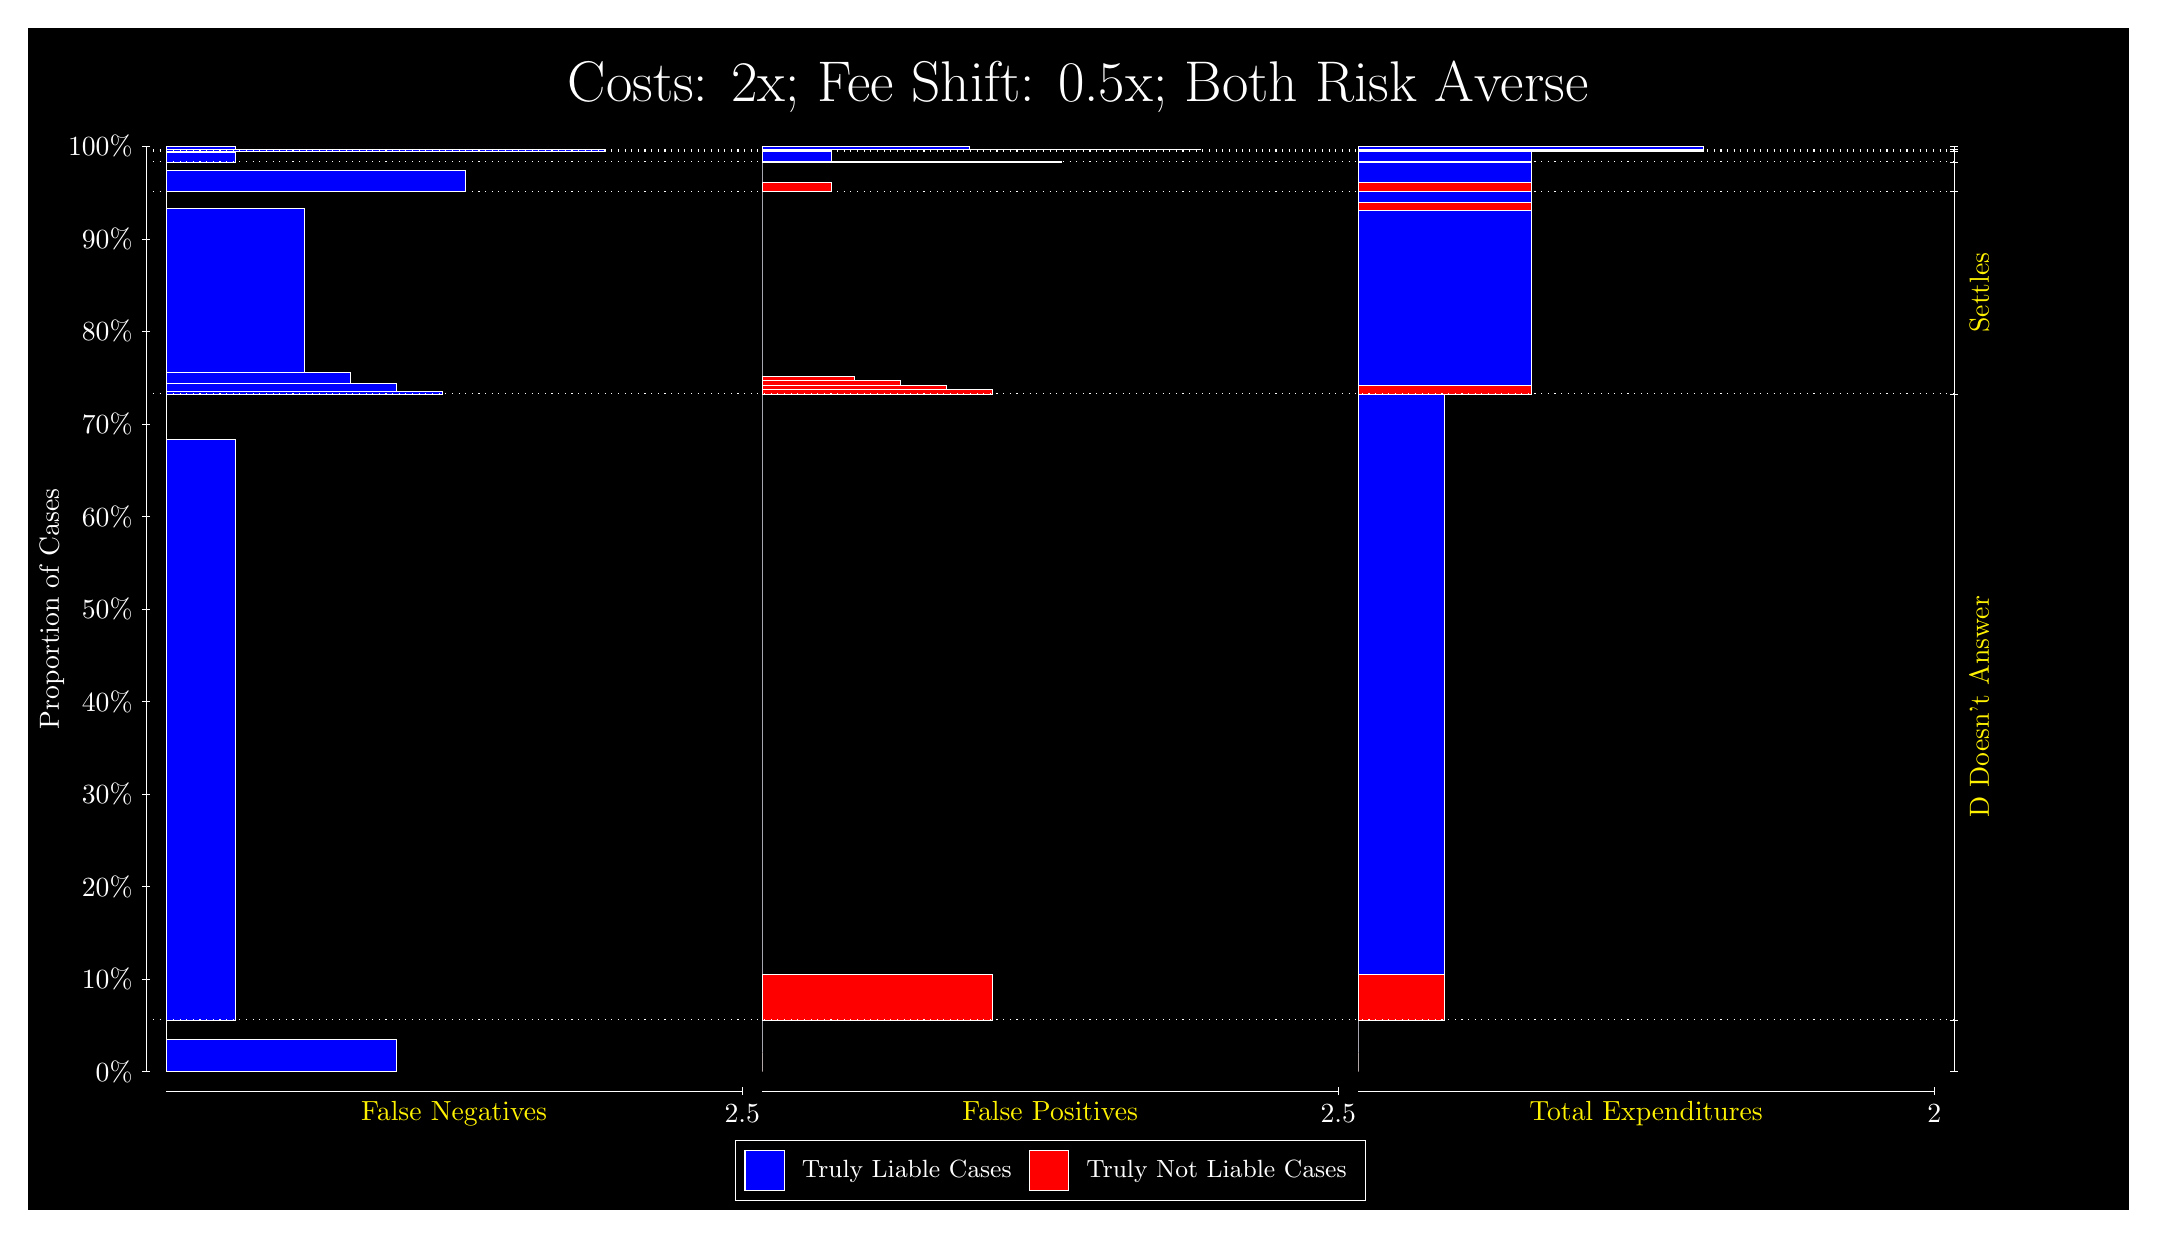
\begin{tikzpicture}
\draw[fill=black] (0,0) rectangle (26.667,15);
\draw[text=white] (0,13.5) rectangle (26.667,15) node[midway] {\huge Costs: 2x; Fee Shift: 0.5x; Both Risk Averse};
\draw[white, very thin] (1.5,1.75) -- (1.5,13.5);
\node[rotate=90, text=white, anchor=center] at (0.3, 7.625) {Proportion of Cases};
\draw[white, very thin] (1.45,1.75) -- (1.55,1.75);
\node[text=white, anchor=east] at (1.45, 1.75) {0\%};
\draw[white, very thin] (1.45,2.925) -- (1.55,2.925);
\node[text=white, anchor=east] at (1.45, 2.925) {10\%};
\draw[white, very thin] (1.45,4.1) -- (1.55,4.1);
\node[text=white, anchor=east] at (1.45, 4.1) {20\%};
\draw[white, very thin] (1.45,5.275) -- (1.55,5.275);
\node[text=white, anchor=east] at (1.45, 5.275) {30\%};
\draw[white, very thin] (1.45,6.45) -- (1.55,6.45);
\node[text=white, anchor=east] at (1.45, 6.45) {40\%};
\draw[white, very thin] (1.45,7.625) -- (1.55,7.625);
\node[text=white, anchor=east] at (1.45, 7.625) {50\%};
\draw[white, very thin] (1.45,8.8) -- (1.55,8.8);
\node[text=white, anchor=east] at (1.45, 8.8) {60\%};
\draw[white, very thin] (1.45,9.975) -- (1.55,9.975);
\node[text=white, anchor=east] at (1.45, 9.975) {70\%};
\draw[white, very thin] (1.45,11.15) -- (1.55,11.15);
\node[text=white, anchor=east] at (1.45, 11.15) {80\%};
\draw[white, very thin] (1.45,12.325) -- (1.55,12.325);
\node[text=white, anchor=east] at (1.45, 12.325) {90\%};
\draw[white, very thin] (1.45,13.5) -- (1.55,13.5);
\node[text=white, anchor=east] at (1.45, 13.5) {100\%};

\draw[white, very thin] (24.457,1.75) -- (24.457,13.5);
\draw[white, very thin] (24.407,1.75) -- (24.507,1.75);
\node[anchor=west] at (24.407, 1.75) {};
\draw[white, very thin] (24.407,2.4071) -- (24.507,2.4071);
\node[anchor=west] at (24.407, 2.4071) {};
\draw[white, very thin] (24.407,10.356) -- (24.507,10.356);
\node[anchor=west] at (24.407, 10.356) {};
\draw[white, very thin] (24.407,12.93) -- (24.507,12.93);
\node[anchor=west] at (24.407, 12.93) {};
\draw[white, very thin] (24.407,13.303) -- (24.507,13.303);
\node[anchor=west] at (24.407, 13.303) {};
\draw[white, very thin] (24.407,13.44) -- (24.507,13.44);
\node[anchor=west] at (24.407, 13.44) {};
\draw[white, very thin] (24.407,13.463) -- (24.507,13.463);
\node[anchor=west] at (24.407, 13.463) {};
\draw[white, very thin] (24.407,13.5) -- (24.507,13.5);
\node[anchor=west] at (24.407, 13.5) {};

\draw[white, very thin, fill=blue] (1.75,1.75) rectangle (4.6775,2.1644);
\draw[white, very thin, fill=red] (1.75,2.1644) rectangle (1.75,2.4071);
\draw[white, very thin, fill=blue] (1.75,2.4071) rectangle (2.6283,9.7737);
\draw[white, very thin, fill=red] (1.75,9.7737) rectangle (1.75,10.356);
\draw[white, very thin, fill=blue] (1.75,10.356) rectangle (5.2631,10.385);
\draw[white, very thin, fill=blue] (1.75,10.385) rectangle (4.9703,10.387);
\draw[white, very thin, fill=blue] (1.75,10.387) rectangle (4.6775,10.491);
\draw[white, very thin, fill=blue] (1.75,10.491) rectangle (4.092,10.632);
\draw[white, very thin, fill=blue] (1.75,10.632) rectangle (3.5065,12.711);
\draw[white, very thin, fill=red] (1.75,12.711) rectangle (1.75,12.93);
\draw[white, very thin, fill=blue] (1.75,12.93) rectangle (5.5558,13.19);
\draw[white, very thin, fill=red] (1.75,13.19) rectangle (1.75,13.303);
\draw[white, very thin, fill=blue] (1.75,13.303) rectangle (2.6283,13.428);
\draw[white, very thin, fill=red] (1.75,13.428) rectangle (1.75,13.44);
\draw[white, very thin, fill=blue] (1.75,13.44) rectangle (7.3123,13.459);
\draw[white, very thin, fill=red] (1.75,13.459) rectangle (1.75,13.463);
\draw[white, very thin, fill=blue] (1.75,13.463) rectangle (2.6283,13.498);
\draw[white, very thin, fill=red] (1.75,13.498) rectangle (1.75,13.5);
\draw[white, very thin, fill=red] (9.3189,1.75) rectangle (9.3189,1.9927);
\draw[white, very thin, fill=blue] (9.3189,1.9927) rectangle (9.3189,2.4071);
\draw[white, very thin, fill=red] (9.3189,2.4071) rectangle (12.246,2.9891);
\draw[white, very thin, fill=blue] (9.3189,2.9891) rectangle (9.3189,10.356);
\draw[white, very thin, fill=red] (9.3189,10.356) rectangle (12.246,10.412);
\draw[white, very thin, fill=red] (9.3189,10.412) rectangle (11.661,10.465);
\draw[white, very thin, fill=red] (9.3189,10.465) rectangle (11.075,10.527);
\draw[white, very thin, fill=red] (9.3189,10.527) rectangle (10.783,10.528);
\draw[white, very thin, fill=red] (9.3189,10.528) rectangle (10.49,10.575);
\draw[white, very thin, fill=blue] (9.3189,10.575) rectangle (9.3189,12.93);
\draw[white, very thin, fill=red] (9.3189,12.93) rectangle (10.197,13.043);
\draw[white, very thin, fill=blue] (9.3189,13.043) rectangle (9.3189,13.303);
\draw[white, very thin, fill=red] (9.3189,13.303) rectangle (13.125,13.314);
\draw[white, very thin, fill=blue] (9.3189,13.314) rectangle (10.197,13.44);
\draw[white, very thin, fill=red] (9.3189,13.44) rectangle (10.197,13.444);
\draw[white, very thin, fill=blue] (9.3189,13.444) rectangle (9.3189,13.463);
\draw[white, very thin, fill=red] (9.3189,13.463) rectangle (14.881,13.465);
\draw[white, very thin, fill=blue] (9.3189,13.465) rectangle (11.954,13.5);
\draw[white, very thin, fill=red] (16.888,1.75) rectangle (16.888,1.9927);
\draw[white, very thin, fill=blue] (16.888,1.9927) rectangle (16.888,2.4071);
\draw[white, very thin, fill=red] (16.888,2.4071) rectangle (17.986,2.9891);
\draw[white, very thin, fill=blue] (16.888,2.9891) rectangle (17.986,10.356);
\draw[white, very thin, fill=red] (16.888,10.356) rectangle (19.083,10.465);
\draw[white, very thin, fill=blue] (16.888,10.465) rectangle (19.083,12.686);
\draw[white, very thin, fill=red] (16.888,12.686) rectangle (19.083,12.795);
\draw[white, very thin, fill=blue] (16.888,12.795) rectangle (19.083,12.93);
\draw[white, very thin, fill=red] (16.888,12.93) rectangle (19.083,13.043);
\draw[white, very thin, fill=blue] (16.888,13.043) rectangle (19.083,13.303);
\draw[white, very thin, fill=red] (16.888,13.303) rectangle (19.083,13.314);
\draw[white, very thin, fill=blue] (16.888,13.314) rectangle (19.083,13.44);
\draw[white, very thin, fill=red] (16.888,13.44) rectangle (21.279,13.444);
\draw[white, very thin, fill=blue] (16.888,13.444) rectangle (21.279,13.463);
\draw[white, very thin, fill=red] (16.888,13.463) rectangle (21.279,13.465);
\draw[white, very thin, fill=blue] (16.888,13.465) rectangle (21.279,13.5);
\draw[white, dotted] (1.5,2.4071) -- (24.457,2.4071);
\draw[white, dotted] (1.5,10.356) -- (24.457,10.356);
\draw[white, dotted] (1.5,12.93) -- (24.457,12.93);
\draw[white, dotted] (1.5,13.303) -- (24.457,13.303);
\draw[white, dotted] (1.5,13.44) -- (24.457,13.44);
\draw[white, dotted] (1.5,13.463) -- (24.457,13.463);
\draw[white, very thin] (1.75,1.5) -- (9.0689,1.5);
\node[text=yellow, anchor=north] at (5.4094, 1.5) {False Negatives};
\draw[white, very thin] (9.0689,1.45) -- (9.0689,1.55);
\node[text=white, anchor=north] at (9.0689, 1.45) {2.5};

\draw[white, very thin] (9.3189,1.5) -- (16.638,1.5);
\node[text=yellow, anchor=north] at (12.978, 1.5) {False Positives};
\draw[white, very thin] (16.638,1.45) -- (16.638,1.55);
\node[text=white, anchor=north] at (16.638, 1.45) {2.5};

\draw[white, very thin] (16.888,1.5) -- (24.207,1.5);
\node[text=yellow, anchor=north] at (20.547, 1.5) {Total Expenditures};
\draw[white, very thin] (24.207,1.45) -- (24.207,1.55);
\node[text=white, anchor=north] at (24.207, 1.45) {2};


\node[text=yellow, centered, rotate=90] at (24.777, 6.3814) {D Doesn't Answer};
\node[text=yellow, centered, rotate=90] at (24.777, 11.643) {Settles};





\draw (12.978300999999998,1.5) node[draw=none] (baseCoordinate) {};
\begin{scope}[align=center]
        \matrix[scale=0.5, draw=white, below=0.5cm of baseCoordinate, nodes={draw}, column sep=0.1cm]{
            \node[rectangle, draw, minimum width=0.5cm, minimum height=0.5cm, fill=blue] {}; &
            \node[draw=none, font=\small, text=white] (B) {Truly Liable Cases}; &
            \node[rectangle, draw, minimum width=0.5cm, minimum height=0.5cm, fill=red] {}; &
            \node[draw=none, font=\small, text=white] (B) {Truly Not Liable Cases}; \\
            };
\end{scope}

\end{tikzpicture}
\end{document}